%%% Analyse for design af snubber-kredsløb til MOSFET og diode %%%

\section{Snubber-kredsløb}
Under 2. iteration blev det observeret under switching, blev der anslået svingninger på spændingen over både MOSFET'en og dioden. Disse højfrekvente svingninger vil, kunne støje på omkringliggende elektronik, både på printet og i rummet. Figur~\ref{fig:MOSFET_svingninger_2} og \ref{fig:diode_svingninger_2} viser problematikken i henholdsvis MOSFET og diode. Her er svingningerne i MOSFET'en tidligere blevet aflæst til at have en frekvens på $25M\hertz$, og svingningerne i dioden til at have en frekvens på $28.57M\hertz$. 

\begin{figure}[H]
	\center
	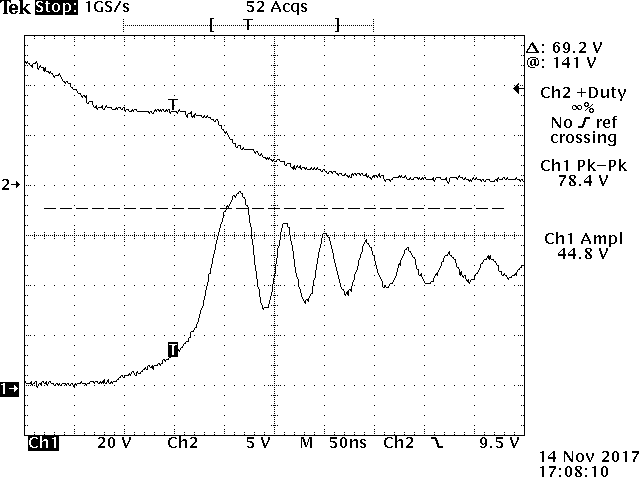
\includegraphics[max width=0.7\linewidth]{/tex/2iteration/billeder/Realisering/Transformator_Primarzoom.PNG}
	\caption{Svingninger i MOSFET}
	\label{fig:MOSFET_svingninger_2}
\end{figure}

\begin{figure}[H]
	\center
	\includegraphics[max width=0.7\linewidth]{/tex/2iteration/billeder/Realisering/Transformator_sekundarzoomrise.PNG}
	\caption{Svingninger i diode}
	\label{fig:diode_svingninger_2}
\end{figure}


Disse svingninger opstår som et biprodukt mellem spredningsselvinduktionen i transformatoren og kapaciteterne i henholdsvis MOSFET og diode. Den kapacitive kobling i transformatoren vil også have en påvirkning på frekvensen af svingningerne. De parasitiske komponenter er indtegnet på figur~\ref{fig:snubber_parasit}\cite{snubber_parasit}.  

\begin{figure}[H]
	\center
	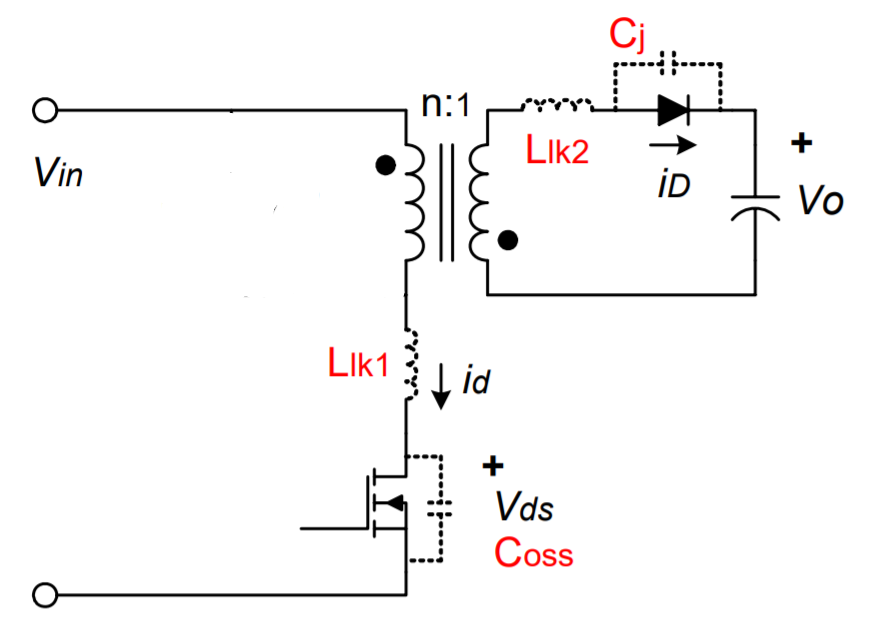
\includegraphics[max width=0.7\linewidth]{/tex/3iteration/billeder/Analyse/snubber_parasit.PNG}
	\caption{Parasitter i MOSFET, diode og transformator}
	\label{fig:snubber_parasit}
\end{figure}

Princippet i et snubber-kredsløb er, at udligne svingningerne med en kondensator, samt bruge en modstand til, at afsætte effekten fra svingningerne i. Derfor vil en konsekvens af, at bruge snubber-kredsløb være et større tab. Det er dog et nødvendigt tab for ikke at generere højfrekvent støj. 

Der er generelt to forskellige snubber-kredsløb der bliver brugt til, at fjerne disse svingninger - en RC-snubber og en RCD-snubber\cite{snubber_design}. En RC-snubber er en modstand og en kondensator i serie. Den bliver primært brugt til at fjerne svingningerne over dioden, men kan også bruges på MOSFET'en. Denne form for snubber er simpel at designe når man kender spredningsselvinduktionen i transformatoren, og er tilstrækkelig til at fjerne svingningerne. En RCD-snubber er en diode placeret i serie med en parallelforbindelse mellem en kondensator og en modstand. Den bruges ofte kun på primærsiden og er placeret over transformatorviklingen. Denne form for snubber er mere kompliceret at designe, og kræver flere komponenter. Derfor vælges det at bruge RC-snubbere på både primær- og sekundærsiden.

Det startes med, at designe kredsløbet til MOSFET'en. Her blev svingningerne aflæst til en frekvens på $25M\hertz$. Ved at bruge spredningsselvinduktionen i transformatoren og svingningsfrekvensen, kan den resulterende kapacitet regnes ved, at løse følgende ligning.
\begin{equation} \label{eq:MOSFET_snubber}
f = \frac{1}{2 \cdot \pi \cdot \sqrt{L_{m} \cdot C_{pri}}} \Rightarrow C_{pri}=266.6pF
\end{equation}

Kondensatoren i snubber kredsløbet bør være ca. $2-3$ gange større end den beregnede kapacitet\cite{snubber_design}. Der vælges en faktor 2:
\begin{equation}
C_{snubM} = 2 \cdot C_{pri} = 533.6pF
\end{equation}

\noindent Det vælges at runde op til $600pF$, da denne værdi kan realiseres. For optimal dæmpning bør impedansen af modstanden, være lig impedansen i spredningsselvinduktionen, ved svingningsfrekvensen. 
\begin{equation}
R_{snubM} = 2 \cdot \pi \cdot L_m \cdot f = 2 \cdot \pi \cdot 152nH \cdot 25M\hertz = 23.9\ohm
\end{equation}

\noindent Her rundes ned til $23.7\ohm$ da denne kan realiseres. 

\noindent For design af snubber-kredsløbet til dioden bruges samme fremgangsmåde.
\begin{equation} \label{eq:diode_snubber}
f = \frac{1}{2 \cdot \pi \cdot \sqrt{L_{m} \cdot C_{sek}}} \Rightarrow C_{sek}=204.1pF
\end{equation}

Igen vælges det, at gøre $C_{snubD}$ en faktor 2 større end $C_{sek}$:
\begin{equation}
C_{snubD} = 2 \cdot C_{sek} = 408.2pF
\end{equation}

\noindent Det vælges at runde ned til $400pF$, da denne værdi kan realiseres. Modstanden dimensioneres ud fra impedansen i spredningsslevinduktionen. 
\begin{equation}
R_{snubD} = 2 \cdot \pi \cdot L_m \cdot f = 2 \cdot \pi \cdot 152nH \cdot 28.6M\hertz = 27.3\ohm
\end{equation}

\noindent Her rundes op til $27.4\ohm$ da denne kan realiseres.


